
\subsection{Focus Area - When}
\textbf{Goal:} Understand when contributions from organizations and people are happening
\begin{table}[ht!]
    \centering
    \begin{tabular}{|p{0.35\linewidth} | p{0.6\linewidth}|}
        \hline
        \hfil \textbf{Metric}  & \hfil \textbf{Question} \\
        \hline
		Activity Dates and Times & What are the dates and timestamps of when contributor activities occur? \\ 
		\hline
		Burstiness & How are short timeframes of intense activity, followed by a corresponding return to a typical pattern of activity, observed in a project? \\ 
		\hline
		Review Cycle Duration within a Change Request & What is the duration of a review cycle within a single change request? \\ 
		\hline
		Time to Close & How much time passes between creating and closing an operation such as an issue, change request, or support ticket? \\ 
		\hline
		Time to First Response & How much time passes between when an activity requiring attention is created and the first response? \\ 
		\hline
    \end{tabular}
\end{table}

\hypertarget{activity-dates-and-times}{%
\section{Activity Dates and Times}\label{activity-dates-and-times}}

Question: What are the dates and timestamps of when contributor
activities occur?

\hypertarget{description}{%
\subsection{Description}\label{description}}

Individuals engage in activities in open source projects at various
times of the day. This metric is aimed at determining the dates and
times of when individual activities were completed. The data can be used
to probabilistically estimate where on earth contributions come from in
cases where the time zone is not UTC.

\hypertarget{objectives}{%
\subsection{Objectives}\label{objectives}}

\begin{itemize}
\tightlist
\item
  Improve transparency for employers about when organizational employees
  are engaging with open source projects
\item
  Improve transparency for open source project and community managers as
  to when activity is occurring
\end{itemize}

\hypertarget{implementation}{%
\subsection{Implementation}\label{implementation}}

\hypertarget{filters}{%
\subsubsection{Filters}\label{filters}}

\begin{itemize}
\tightlist
\item
  Individual by Organization
\item
  Aggregation of time by UTC time

  \begin{itemize}
  \tightlist
  \item
    Can show what times across the globe contributions are made; when
    the project is most active.
  \end{itemize}
\item
  Aggregation of time by local time

  \begin{itemize}
  \tightlist
  \item
    Can show what times of day in their local times they contribute.
    Conclusions about the If contributions are more during working
    hours, or if contributions are more during evening hours.
  \end{itemize}
\item
  Repository ID
\item
  Segment of a community, (e.g., GrimoireLab has more EU time zones
  activity and Augur more US time zones activity)
\end{itemize}

\hypertarget{visualizations}{%
\subsubsection{Visualizations}\label{visualizations}}

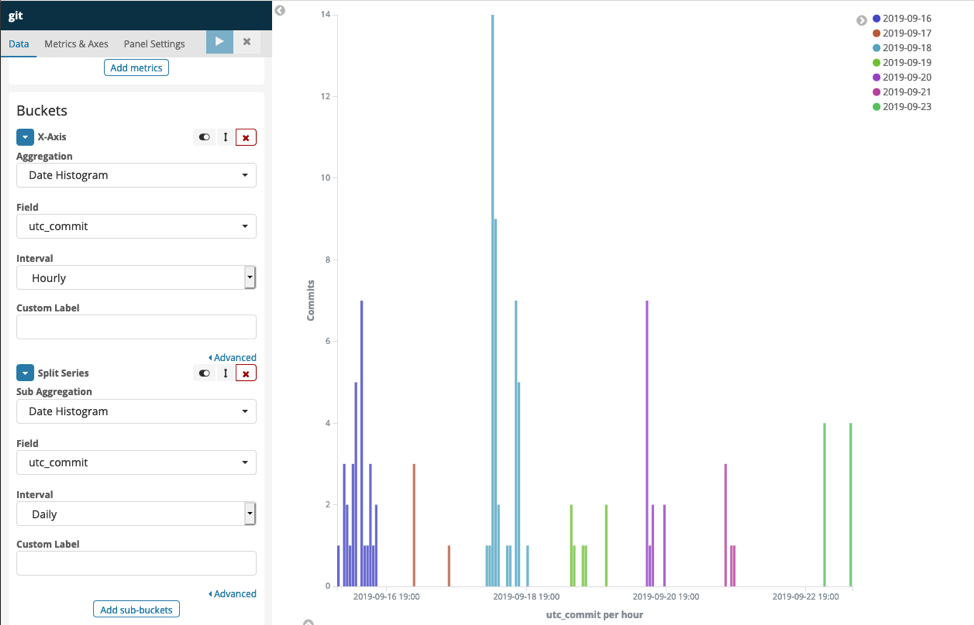
\includegraphics{images/activity-dates-and-times_1.png}
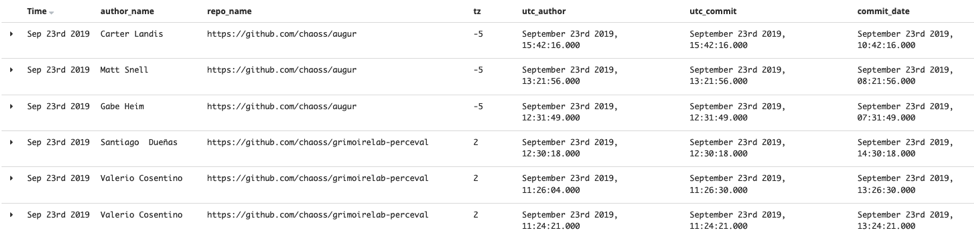
\includegraphics{images/activity-dates-and-times_2.png}
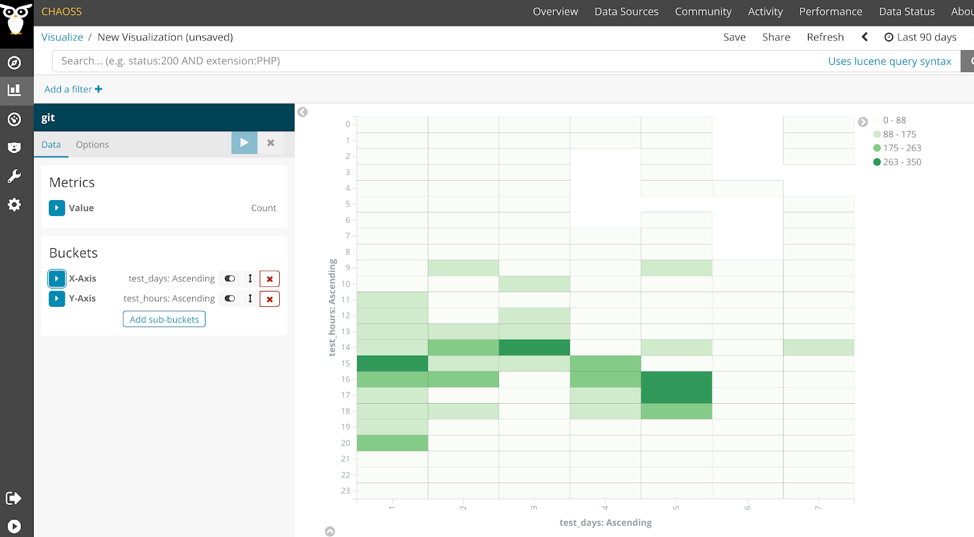
\includegraphics{images/activity-dates-and-times_3.png}
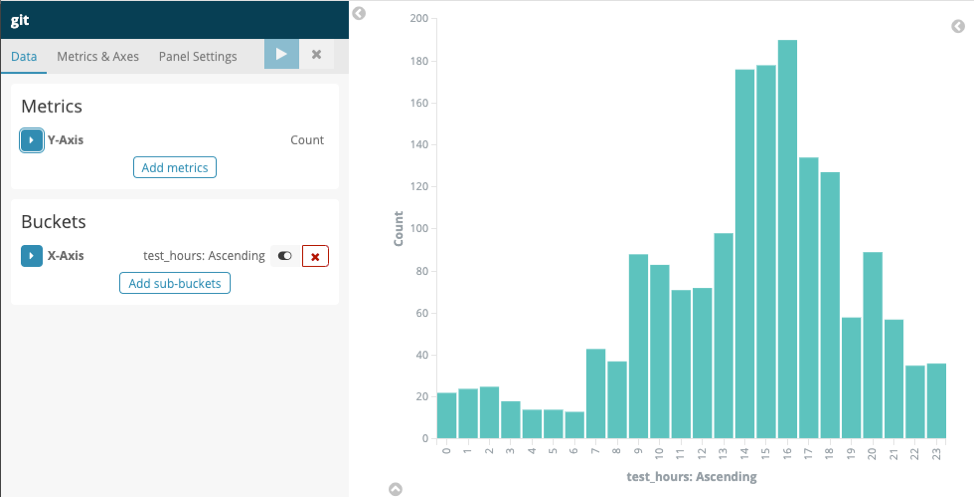
\includegraphics{images/activity-dates-and-times_4.png}

\hypertarget{tools-providing-metric}{%
\subsubsection{Tools Providing Metric}\label{tools-providing-metric}}

\href{https://chaoss.github.io/grimoirelab/}{GrimoireLab}

\href{https://docs.augur.net/\#dates-timestamps}{Augur Date/Timestamps}

\hypertarget{references}{%
\subsection{References}\label{references}}

\href{https://en.wikipedia.org/wiki/Coordinated_Universal_Time}{Coordinated
Universal Time}
 
\hypertarget{burstiness}{%
\section{Burstiness}\label{burstiness}}

Question: How are short timeframes of intense activity, followed by a
corresponding return to a typical pattern of activity, observed in a
project?

\hypertarget{description}{%
\subsection{Description}\label{description}}

There are a number of reasons that may prompt a sudden increase or
decrease in the amount of activity within a repository. These increases
and decreases appear both as a sudden change in activity against the
average amount of activity. Burstiness is a way of understanding the
cycle of activity in existing metrics, like issues, merge requests,
mailing lists, commits, or comments. Examples of root causes for bursts
in activity include:

\begin{itemize}
\tightlist
\item
  Release cycles
\item
  Global pandemics
\item
  Hackathon activities
\item
  Mentorship programs
\item
  Conferences, meetups, and other events where tools are presented
\item
  Conventional and social media announcements and mentions
\item
  Critical bugs as raising awareness and getting people's attention
\item
  Community design meetings or brainstorming meetings to address a
  particular issue
\item
  Community members show up from another community that is relying on
  your project (e.g., dependencies)
\end{itemize}

\hypertarget{objectives}{%
\subsection{Objectives}\label{objectives}}

\begin{itemize}
\tightlist
\item
  To identify impacts of root causes of a burst in activity
\item
  To provide awareness when project activity unknowingly goes up
\item
  To help capture the meaningfulness of increases or decreases in
  project activity
\item
  To help the community and maintainers prepare for future bursts that
  follow a pattern
\item
  To help measure the impact of influential external activities
\item
  To differentiate skewed activity versus normal activity
\end{itemize}

\hypertarget{implementation}{%
\subsection{Implementation}\label{implementation}}

\hypertarget{filters}{%
\subsubsection{Filters}\label{filters}}

\begin{itemize}
\tightlist
\item
  Stars
\item
  Forks
\item
  Issues or bug reports
\item
  Labels
\item
  Downloads
\item
  Release Tags
\item
  Change Requests
\item
  Mail List Traffic
\item
  Documentation additions or revisions
\item
  New Repositories
\item
  Feature Requests
\item
  Messaging Conversations
\item
  Conventional and Social Media Activity
\item
  Conference Attendance and Submissions
\end{itemize}

\hypertarget{visualizations}{%
\subsubsection{Visualizations}\label{visualizations}}

Augur:

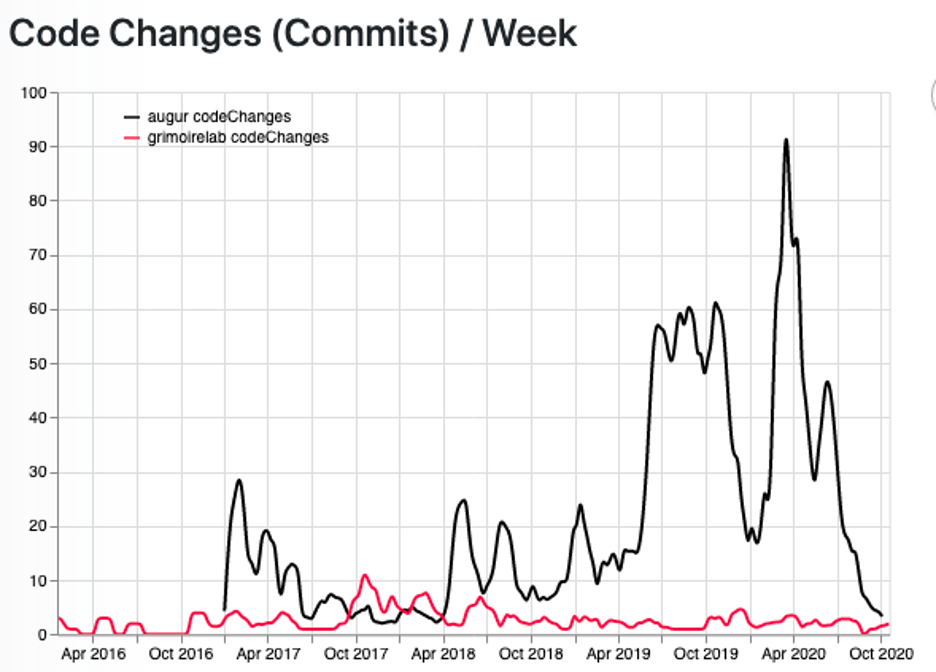
\includegraphics{images/burstiness_augur.png}

GrimoireLab:

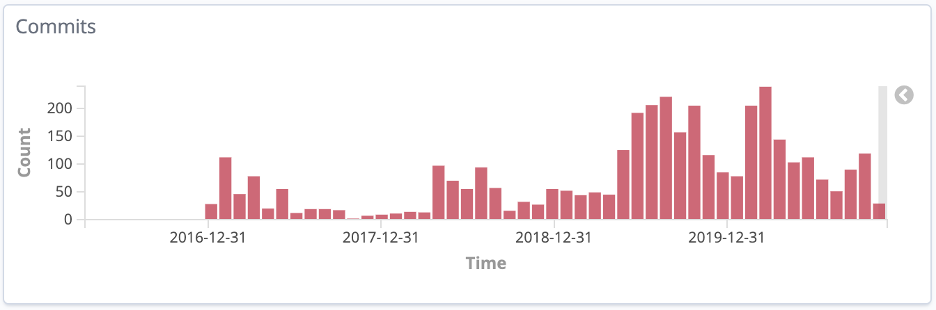
\includegraphics{images/burstiness_gl.png}

\hypertarget{tools-providing-the-metric}{%
\subsubsection{Tools Providing the
Metric}\label{tools-providing-the-metric}}

\begin{itemize}
\tightlist
\item
  Grimoire Lab
\item
  Augur
\end{itemize}

\hypertarget{data-collection-strategies}{%
\subsubsection{Data Collection
Strategies}\label{data-collection-strategies}}

\begin{itemize}
\item
  Quantitative

  \begin{itemize}
  \tightlist
  \item
    Time box activities identifying deviations away from some norm
  \item
    Outliers for certain thresholds, using statistics like Bollinger
    Bands to measure stability or volatility:
    \url{https://en.wikipedia.org/wiki/Bollinger_Bands}
  \end{itemize}
\item
  Qualitative Interview Questions

  \begin{itemize}
  \tightlist
  \item
    Why do you contribute more during a period of time?
  \item
    What do you believe to be the root cause for particular bursts?
  \item
    What impact do different events (e.g., hackathons, mentorship
    program, or conferences) have on project activity?
  \end{itemize}
\end{itemize}

\hypertarget{references}{%
\subsection{References}\label{references}}

This metric was inspired by the work of Goh and Barabasi (2008):
\url{https://arxiv.org/pdf/physics/0610233.pdf}
 
\hypertarget{review-cycle-duration-within-a-change-request}{%
\subsubsection{Review Cycle Duration within a Change
Request}\label{review-cycle-duration-within-a-change-request}}

Question: What is the duration of a review cycle within a single change
request?

\hypertarget{description}{%
\paragraph{Description}\label{description}}

A change request is based on one or more review cycles. Within a review
cycle, one or more reviewers can provide feedback on a proposed
contribution. The duration of a review cycle, or the time between each
new iteration of the contribution, is the basis of this metric.

\hypertarget{objectives}{%
\paragraph{Objectives}\label{objectives}}

This metric provides maintainers with insight on: Code review process
decay, as there are more iterations and review cycle durations increase.
Process bottlenecks resulting in long code review iterations. Abandoned
or semi-abandoned processes in the review cycles, where either the
maintainer or the submitter is slow in responding. Characteristics of
reviews that have different cyclic pattern lengths.

\hypertarget{implementation}{%
\paragraph{Implementation}\label{implementation}}

Review Cycle Duration is measured as the time length of one review cycle
within a single change request. The duration can be calculated between:
The moment when each review cycle begins, defined as the point in time
when a change request is submitted or updated. The moment when each
review cycle ends, either because the change request was updated and
needs a new review or because it was accepted or rejected.

\hypertarget{filter}{%
\subparagraph{Filter}\label{filter}}

Average or Median Duration, optionally filtered or grouped by: Number of
people involved in review Number of comments in review Edits made to a
change request Project or program Organization making the change request
Time the change request was submitted Developers who contributed to a
change request Change request Number of review cycle on a change request
(e.g., filter by first, second, \ldots{} round)

\hypertarget{visualizations}{%
\subparagraph{Visualizations}\label{visualizations}}

\hypertarget{tools-providing-the-metric}{%
\subparagraph{Tools Providing the
Metric}\label{tools-providing-the-metric}}

\hypertarget{references}{%
\paragraph{References}\label{references}}

Example of data that could be used to develop the metric:
\url{https://gerrit.wikimedia.org/r/c/mediawiki/core/+/194071}
 
\hypertarget{ux5173ux95edux65f6ux957f}{%
\subsubsection{关闭时长}\label{ux5173ux95edux65f6ux957f}}

问题:创建和关闭操作(如议题、更改请求或需要支持的问题单)之间需要多少时间?

\hypertarget{ux63cfux8ff0}{%
\paragraph{描述}\label{ux63cfux8ff0}}

关闭时长是指从创建到关闭操作(如议题、更改请求或需要支持的问题单)的总时长。
操作需要具有打开和关闭的状态,比如代码审查进程、问答论坛、问题跟踪系统中经常出现的情况。

相关指标:\href{https://chaoss.community/metric-issue-resolution-duration/}{问题解决时长}

\hypertarget{ux76eeux6807}{%
\paragraph{目标}\label{ux76eeux6807}}

\begin{enumerate}
\def\labelenumi{\arabic{enumi}.}
\tightlist
\item
  确定社区的响应程度,帮助增加包容性,吸引新贡献者并保留现有贡献者。
\item
  找出导致快速或缓慢关闭的操作特征(如寻找最佳实践、改进领域、评估效率)。
\item
  识别对不同社区成员及时响应的偏差。
\item
  检测社区活动的变化(例如,显示潜在的维护者倦怠、贡献多元化的减少)
\item
  了解关闭议题或更改请求的时间与合并成功或失败的关系
\end{enumerate}

\hypertarget{ux5b9eux73b0}{%
\paragraph{实现}\label{ux5b9eux73b0}}

\hypertarget{ux7b5bux9009ux6761ux4ef6}{%
\subparagraph{筛选条件}\label{ux7b5bux9009ux6761ux4ef6}}

\begin{itemize}
\tightlist
\item
  操作的创建者(例如,新贡献者相对于维护者)
\item
  最初关闭,最后关闭
\item
  标签(例如错误与新功能)
\item
  更改请求合并状态(例如,合并时间或没有合并的关闭时间)
\end{itemize}

\hypertarget{ux53efux89c6ux5316ux6548ux679c}{%
\subparagraph{可视化效果}\label{ux53efux89c6ux5316ux6548ux679c}}

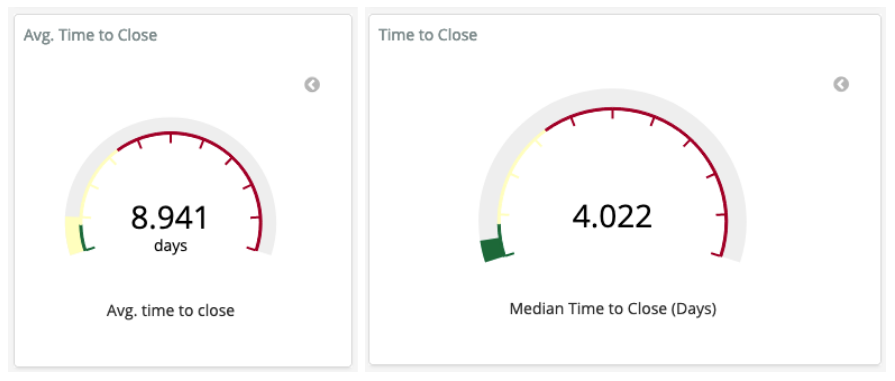
\includegraphics{images/time-to-close_1.png}

\hypertarget{ux63d0ux4f9bux6307ux6807ux7684ux5de5ux5177}{%
\subparagraph{提供指标的工具}\label{ux63d0ux4f9bux6307ux6807ux7684ux5de5ux5177}}

Augur 实现:

\begin{itemize}
\tightlist
\item
  \href{http://augur.osshealth.io/api_docs/\#api-Evolution-Closed_Issue_Resolution_Duration(Repo)}{问题解决时长}
\item
  \href{http://augur.osshealth.io/api_docs/\#api-Evolution-issue-duration-repo}{问题持续时间}
\item
  \href{http://augur.osshealth.io/api_docs/\#api-Evolution-Issue_Response_Time(Repo)}{问题响应时间}
\end{itemize}

GrimoireLab 实现:

\begin{itemize}
\tightlist
\item
  \href{https://chaoss.github.io/grimoirelab-sigils/panels/github-pullrequests-efficiency/}{拉取请求效率}
\item
  \href{https://chaoss.github.io/grimoirelab-sigils/panels/github-issues-efficiency/}{问题效率}
\item
  \href{https://chaoss.github.io/grimoirelab-sigils/panels/efficiency-timing-overview/}{Efficiency:TimingOverview}
\end{itemize}

\hypertarget{ux6570ux636eux6536ux96c6ux7b56ux7565}{%
\subparagraph{数据收集策略}\label{ux6570ux636eux6536ux96c6ux7b56ux7565}}

关闭时长指标可根据项目活动和目标的具体情况而定。
例如,错误报告的关闭时长可能提供与新功能请求的关闭时长不同的信息。
数据收集策略应针对不同的项目目标。 可能影响这些进程的其他变量是:

\begin{itemize}
\tightlist
\item
  问题跟踪系统:如错误报告、蓝图 (OpenStack 专有命名)、用户故事(user
  story)、功能请求、epic等可能会影响事件关闭时长的议题类型。
  优先级或严重性等其他变量可能有助于推进这一事件的关闭速度。
\item
  变更请求流程:这取决于变更请求的平台架构,如 Gerrit、GitHub
  或邮件列表(如 Linux 内核中),并可能根据进程的复杂程度而有所不同。
  例如,新人和经验丰富的高级开发者将以不同的方式开展进程,所需时间或多或少。
\item
  问答论坛:这取决于回答的质量和提问者的意见。
  有效答案会被标记,提问者成功找到自己问题的正确答案后,进程随即关闭。
\end{itemize}

\hypertarget{ux53c2ux8003ux8d44ux6599}{%
\paragraph{参考资料}\label{ux53c2ux8003ux8d44ux6599}}

\begin{itemize}
\tightlist
\item
  ``Practice P.12: Respond to all submissions'',出自``Appendix to:
  Managing Episodic Volunteers in Free/Libre/Open Source Software
  Communities'',Ann Barcomb、Klaas-Jan Stol、Brian Fitzgerald 和 Dirk
  Riehle:\href{https://opus4.kobv.de/opus4-fau/frontdoor/index/index/docId/13519}{https://opus4.kobv.de/opus4-fau/frontdoor/index/index/docId/13519}
\end{itemize}
 
\hypertarget{time-to-first-response}{%
\subsubsection{Time to First Response}\label{time-to-first-response}}

Question: How much time passes between when an activity requiring
attention is created and the first response?

\hypertarget{description}{%
\paragraph{Description}\label{description}}

The first response to an activity can sometimes be the most important
response. The first response shows that a community is active and
engages in conversations. A long time to respond to an activity can be a
sign that a community is not responsive. A short time to respond to an
activity can help to engage more members into further discussions and
within the community.

\hypertarget{objectives}{%
\paragraph{Objectives}\label{objectives}}

Identify cadence of first response across a variety of activities,
including PRs, Issues, emails, IRC posts, etc. Time to first response is
an important consideration for new and long-time contributors to a
project along with overall project health.

\hypertarget{implementation}{%
\paragraph{Implementation}\label{implementation}}

Time to first response of an activity = time first response was posted
to the activity - time the activity was created.

\hypertarget{filters}{%
\subparagraph{Filters}\label{filters}}

\begin{itemize}
\tightlist
\item
  Role of responder, e.g., only count maintainer responses
\item
  Automated responses, e.g., only count replies from real people by
  filtering bots and other automated replies
\item
  Type of Activity, e.g., issues (see metric
  \href{https://github.com/chaoss/wg-evolution/blob/master/metrics/Issue_Response_Time.md}{Issue
  Response Time}), emails, chat, change requests
\end{itemize}

\hypertarget{visualizations}{%
\subparagraph{Visualizations}\label{visualizations}}

<<<<<<< HEAD
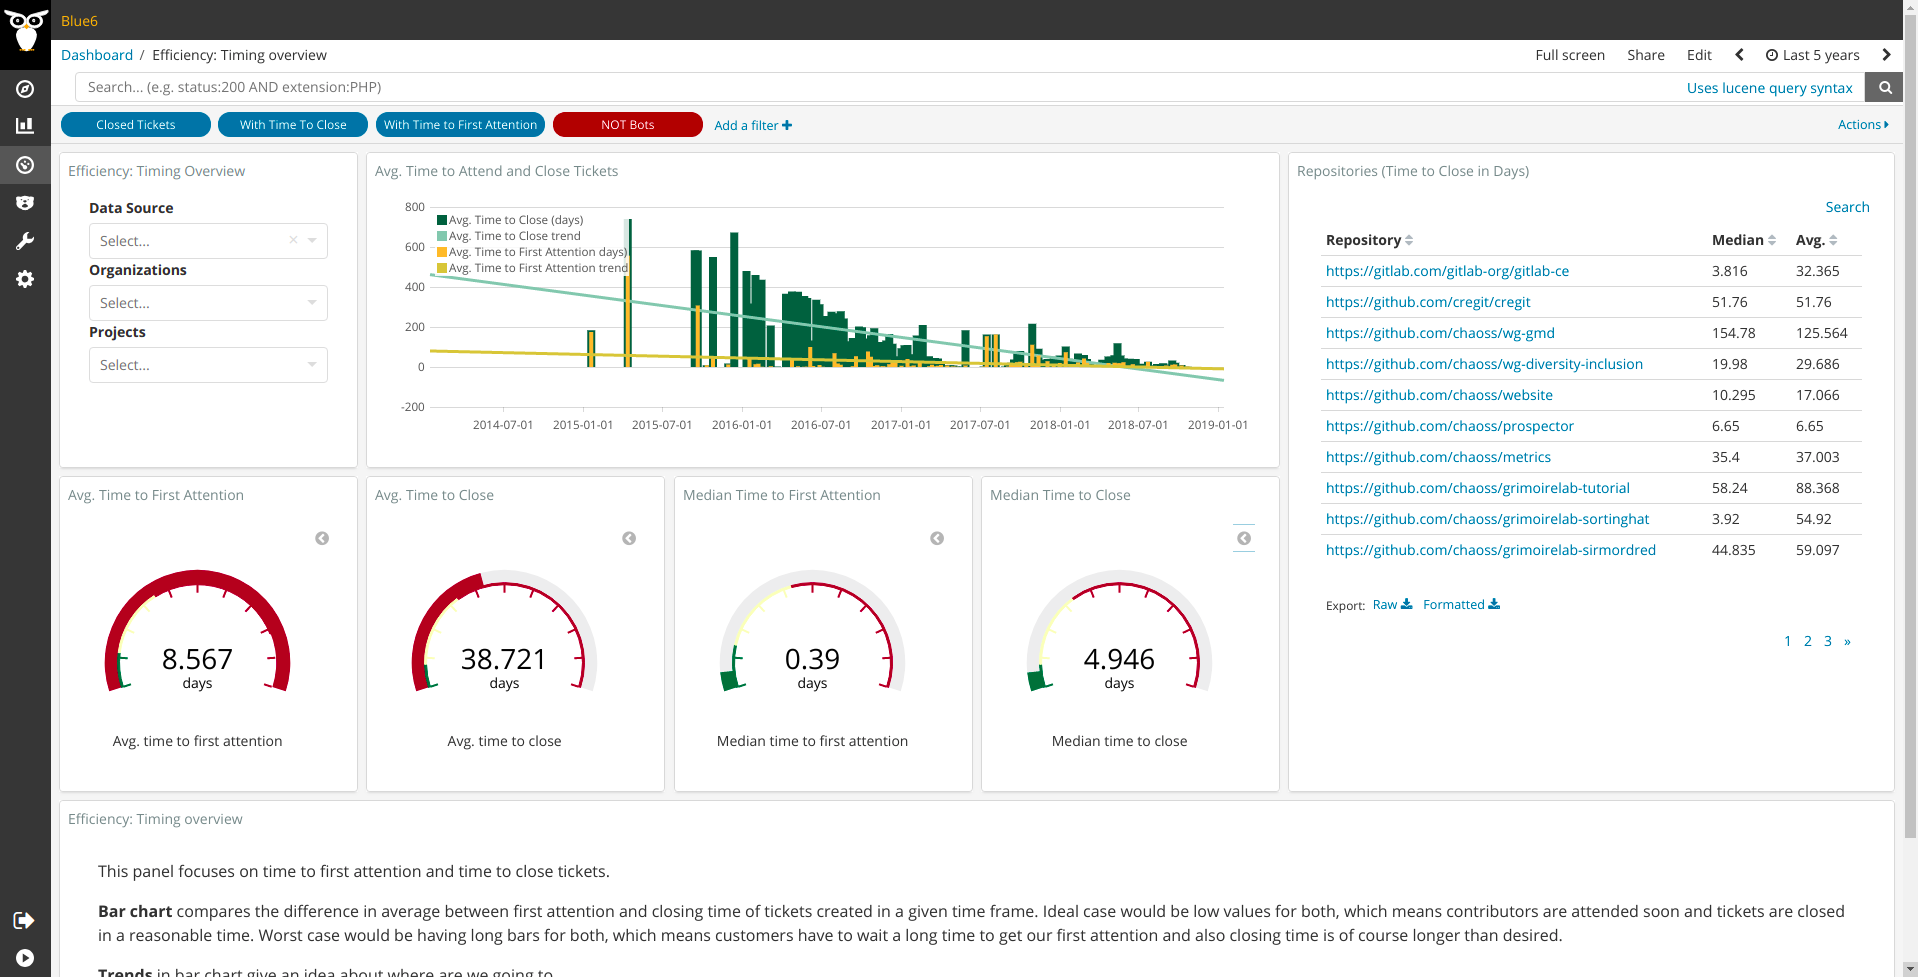
\includegraphics{images/time-to-first-response_efficiency-timing-overview.png}

\begin{center}\rule{0.5\linewidth}{0.5pt}\end{center}

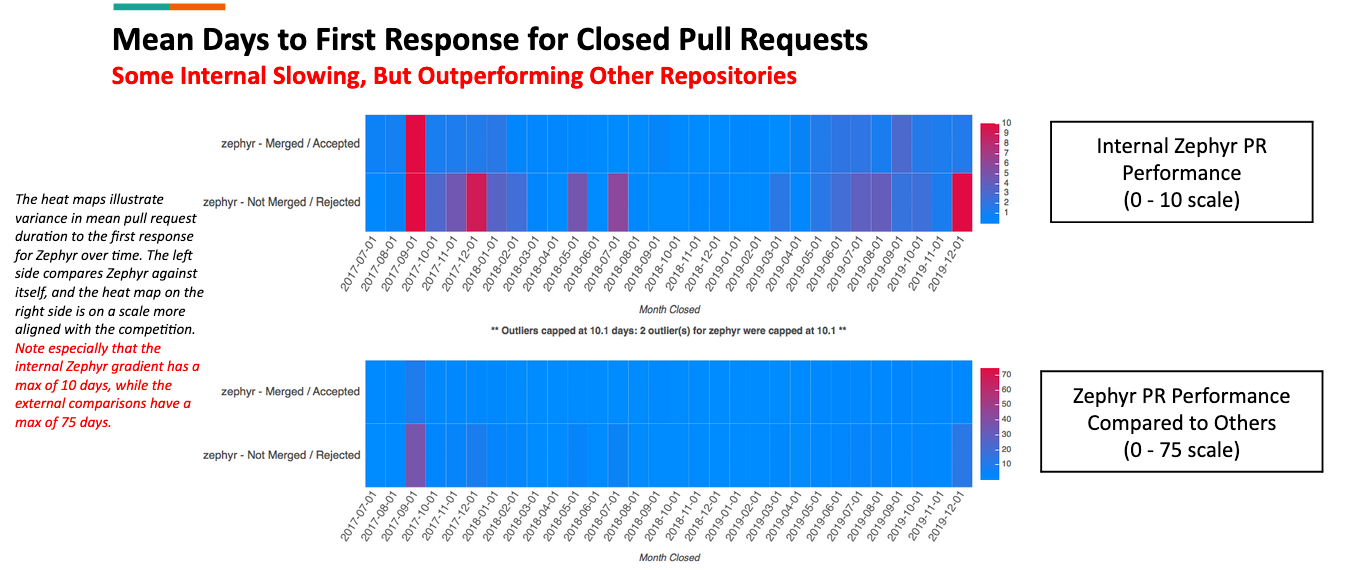
\includegraphics{images/time-to-first-response_augur-ttc-1.png}

\begin{center}\rule{0.5\linewidth}{0.5pt}\end{center}
=======
\hypertarget{grimoirelab-panel-efficiency-timing-overview}{%
\subsection{\texorpdfstring{\protect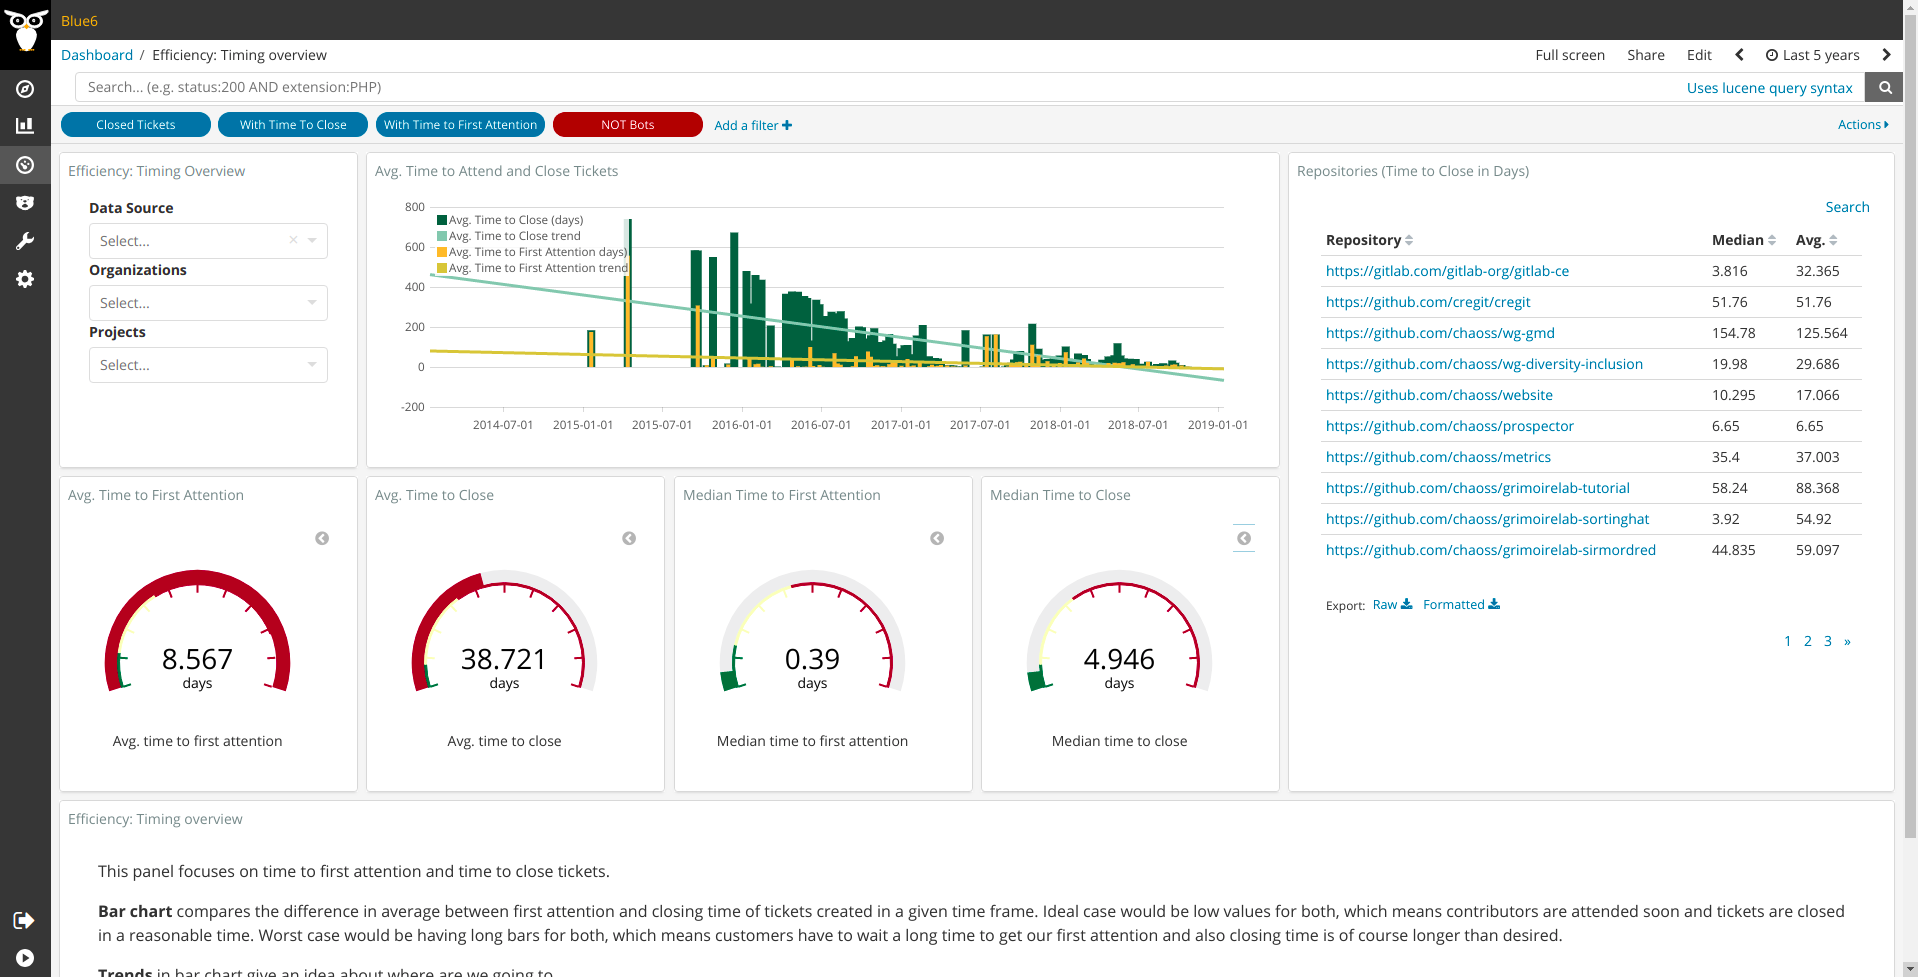
\includegraphics{images/time-to-first-response_efficiency-timing-overview.png}}{GrimoireLab Panel: Efficiency Timing Overview}}\label{grimoirelab-panel-efficiency-timing-overview}}

\hypertarget{augur-visualization-time-to-first-response-heat-map-}{%
\subsection{\texorpdfstring{\protect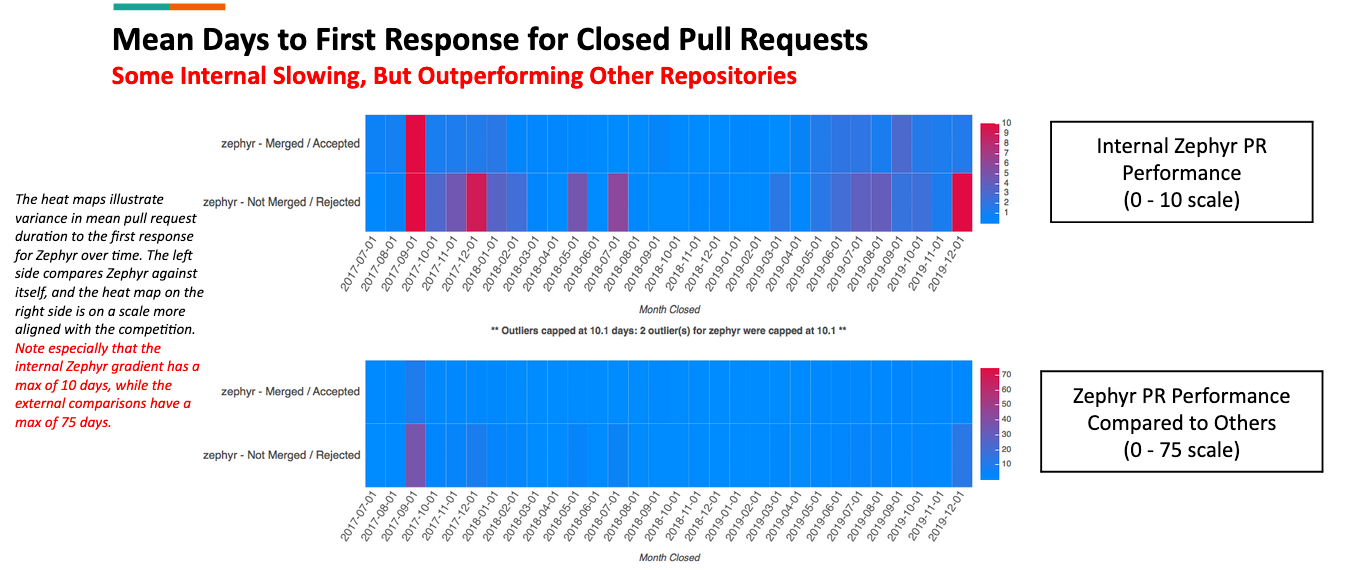
\includegraphics{images/time-to-first-response_augur-ttc-1.png}}{Augur Visualization: Time to First Response Heat Map }}\label{augur-visualization-time-to-first-response-heat-map-}}
>>>>>>> main

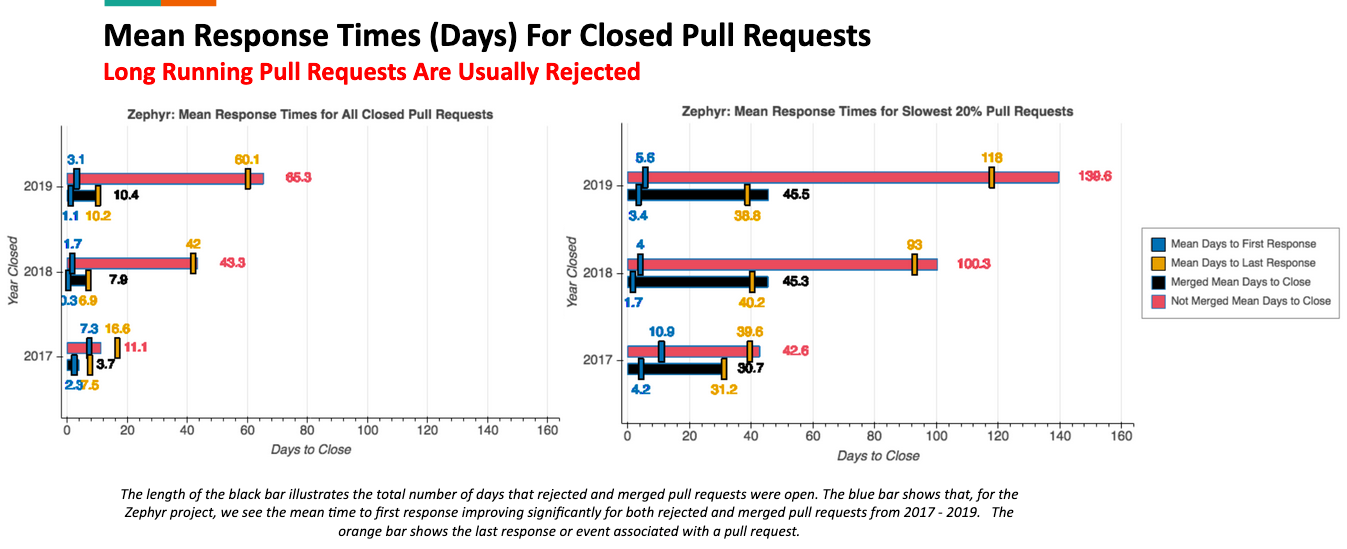
\includegraphics{images/time-to-first-response_augur-ttc-2.png}

\hypertarget{tools-providing-the-metric}{%
\subparagraph{Tools Providing the
Metric}\label{tools-providing-the-metric}}

\begin{itemize}
\tightlist
\item
  GrimoireLab Panel:
  \href{https://chaoss.github.io/grimoirelab-sigils/panels/efficiency-timing-overview/}{Efficiency
  Timing Overview}
\item
  \href{https://katacontainers.biterg.io/app/kibana\#/dashboard/cbbdd920-288c-11e9-b662-975152e57997}{Kata
  Containers dashboard efficiency panel}
\end{itemize}

\hypertarget{references}{%
\paragraph{References}\label{references}}
 
